\begin{figure}[!b]
\begin{center}
 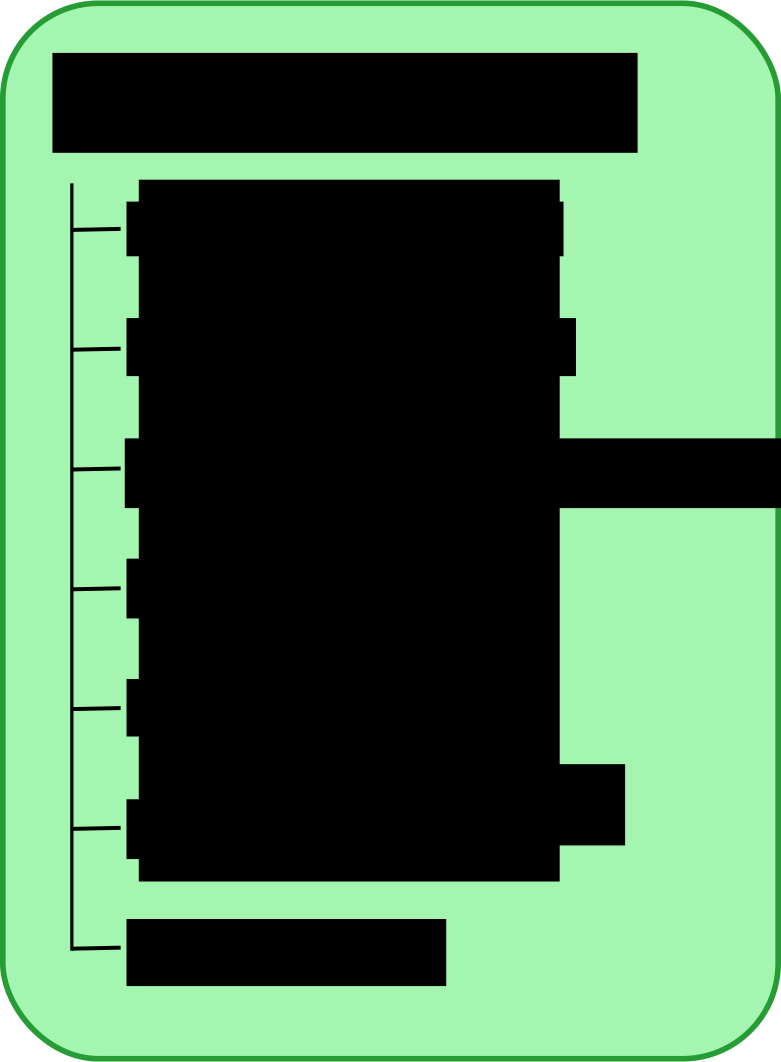
\includegraphics[width=\linewidth/2]{constraint.pdf} \caption{Important methods in Constraint 
class}\label{fig_constraint}
\end{center} 
\end{figure}
Constraints are all derived from the same class (\class{Constraint} figure \ref{fig_constraint}) that forces some 
methods to be implemented. All constraints need a priority according to how important the constraint is, that is an 
integer. The priority do not need to be different for the constraints but it will help the local search to 
differentiate between infeasible  
solutions. \\ 
The method \method{getType} is only used if Gecode does not find an initial solution. How Gecode is used is discussed 
in section \ref{sec_gecode}.   \\ 
An example of a constraint is the \class{Linear} constraint, which is the same as the one used in Integer and binary 
programming, equation \ref{equat_linear} is an example of a \class{Linear} constraint. 
\begin{equation}
 c_1: \; 2x_1 + 2x_2 \leq 2  \qquad x_!,x_2 \in \{0,1\}
\end{equation} \label{equat_linear}
A constraint is posted in the constraint programming environment and later handled in the local search environment. The 
constraints are treated differently in the environments and need different parameters and methods for that. The LS 
environment handles constraints through invariants hence a constraint needs a method for creating the invariants 
needed in LS for the specific type of constraint. The method \method{createInvariants} creates auxiliary 
variables, invariants, that might be auxiliary variables helpful during local search and one invariant that represents 
if the constraint is violated and the cost of being violated. The violation cost can be one if violated and zero 
otherwise, or it give a measurement of violated the constraint is. For the linear constraint $c_1$ in the example the 
measurement could be how much the left hand side should decrease to satisfy the constraint. A helpful auxiliary 
variable is the value of the left hand side such that it does not need to be recomputed when computing the violation. \\
The methods \method{canBeMadeOneway} and \method{makeOneway} are used if the constraint can be transformed 
to a oneway constraint hence functionally define one of the variables. Method \method{canBeMadeOneway} returns a 
boolean whether it can be used or not and \method{makeOneway} returns the oneway constraint, implemented as invariant, 
that defines a variable. For the \class{Linear} constraint only the constraints with an equal relation can be used, 
hence not $c_1$. Why this is done and an example of how is described in section \ref{sec_ls}.